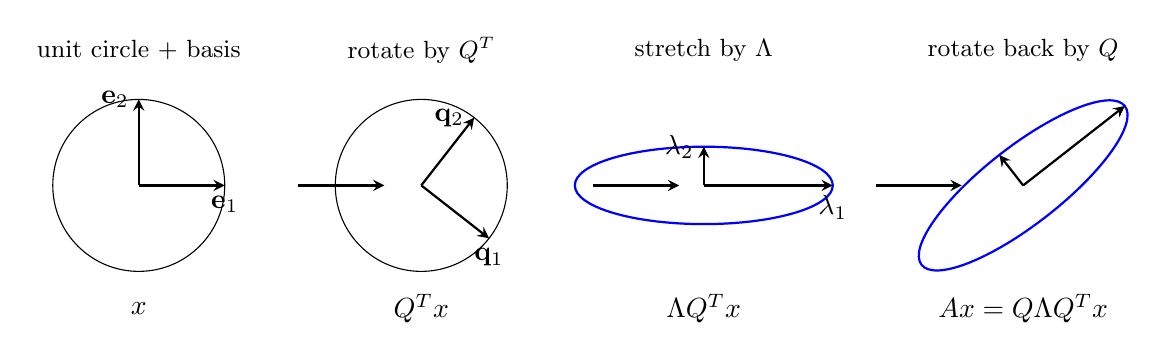
\begin{tikzpicture}[scale=0.78,>=stealth]
\node at (0,2.2) {\small unit circle + basis};
\draw (0,0) circle (1.4);
\draw[->,thick] (0,0)--(1.4,0) node[below]{$\mathbf e_1$};
\draw[->,thick] (0,0)--(0,1.4) node[left]{$\mathbf e_2$};
\node at (0,-2.0) {$x$};
\begin{scope}[xshift=4.6cm]
\node at (0,2.2) {\small rotate by $Q^{T}$};
\begin{scope}[rotate=-38]
\draw (0,0) circle (1.4);
\draw[->,thick] (0,0)--(1.4,0) node[below]{$\mathbf q_1$};
\draw[->,thick] (0,0)--(0,1.4) node[left]{$\mathbf q_2$};
\end{scope}
\node at (0,-2.0) {$Q^{T}x$};
\end{scope}
\begin{scope}[xshift=9.2cm]
\node at (0,2.2) {\small stretch by $\Lambda$};
\draw[blue,thick] (0,0) ellipse (2.1 and 0.63);
\draw[->,thick] (0,0)--(2.1,0) node[below]{$\lambda_1$};
\draw[->,thick] (0,0)--(0,0.63) node[left]{$\lambda_2$};
\node at (0,-2.0) {$\Lambda Q^{T}x$};
\end{scope}
\begin{scope}[xshift=14.4cm]
\node at (0,2.2) {\small rotate back by $Q$};
\begin{scope}[rotate=38]
\draw[blue,thick] (0,0) ellipse (2.1 and 0.63);
\draw[->,thick] (0,0)--(2.1,0);
\draw[->,thick] (0,0)--(0,0.63);
\end{scope}
\node at (0,-2.0) {$Ax=Q\Lambda Q^{T}x$};
\end{scope}
\foreach \xx in {2.6,7.4,12.0} \draw[->,thick] (\xx,0)--(\xx+1.4,0);
\end{tikzpicture}
